\chapter{Curvas Caracteristicas}
    El comportamiento eléctrico del transistor BJT puede representarse mediante sus \textbf{curvas características}, que describen las relaciones entre corrientes y tensiones en sus terminales bajo diferentes condiciones de polarización. Estas curvas permiten identificar claramente las \textit{regiones de operación} del transistor: corte, activa y saturación.
    
    Una de las curvas más representativas es la familia de curvas $I_C$ vs.\ $V_{CE}$ para distintos valores de $I_B$. Estas muestran cómo varía la corriente de colector en función de la tensión colector-emisor, manteniendo constante la corriente de base. Esta representación permite visualizar:
    
    \begin{itemize}
        \item La \textbf{región de corte}: cuando $I_B = 0$, no hay conducción.
        \item La \textbf{región activa}: donde se cumple que $I_C \approx \beta \cdot I_B$.
        \item La \textbf{región de saturación}: donde $V_{CE}$ es bajo y $I_C$ deja de aumentar significativamente.
    \end{itemize}
    
    El análisis experimental de estas curvas, junto con su comparación con resultados simulados y teóricos, permite comprender en profundidad el funcionamiento del transistor y validar su modelo de comportamiento.
\newpage

  \section{Simulacion}
  
    En esta parte se simula el comportamiento del transistor barrando $V_{CE}$ para distintos valores de $I_B$, obteniendo las curvas $I_C$ vs.\ $V_{CE}$. Estas curvas permitieron visualizar claramente las regiones de operación del BJT y validar el modelo teórico mediante comparación con los resultados experimentales.

    %Circuito usado en el simulador con los parametros
    %Grafico de las curvas
    
\newpage

  \section{Laboratorio}

  En esta parte se realizaron mediciones experimentales de la corriente de colector $I_C$ en función de la tensión colector-emisor $V_{CE}$, para distintos valores de corriente de base $I_B$. Esto permitió identificar las regiones de corte, activa y saturación del transistor.

  \begin{figure}[!ht]

        \begin{minipage}{0.5\textwidth}
            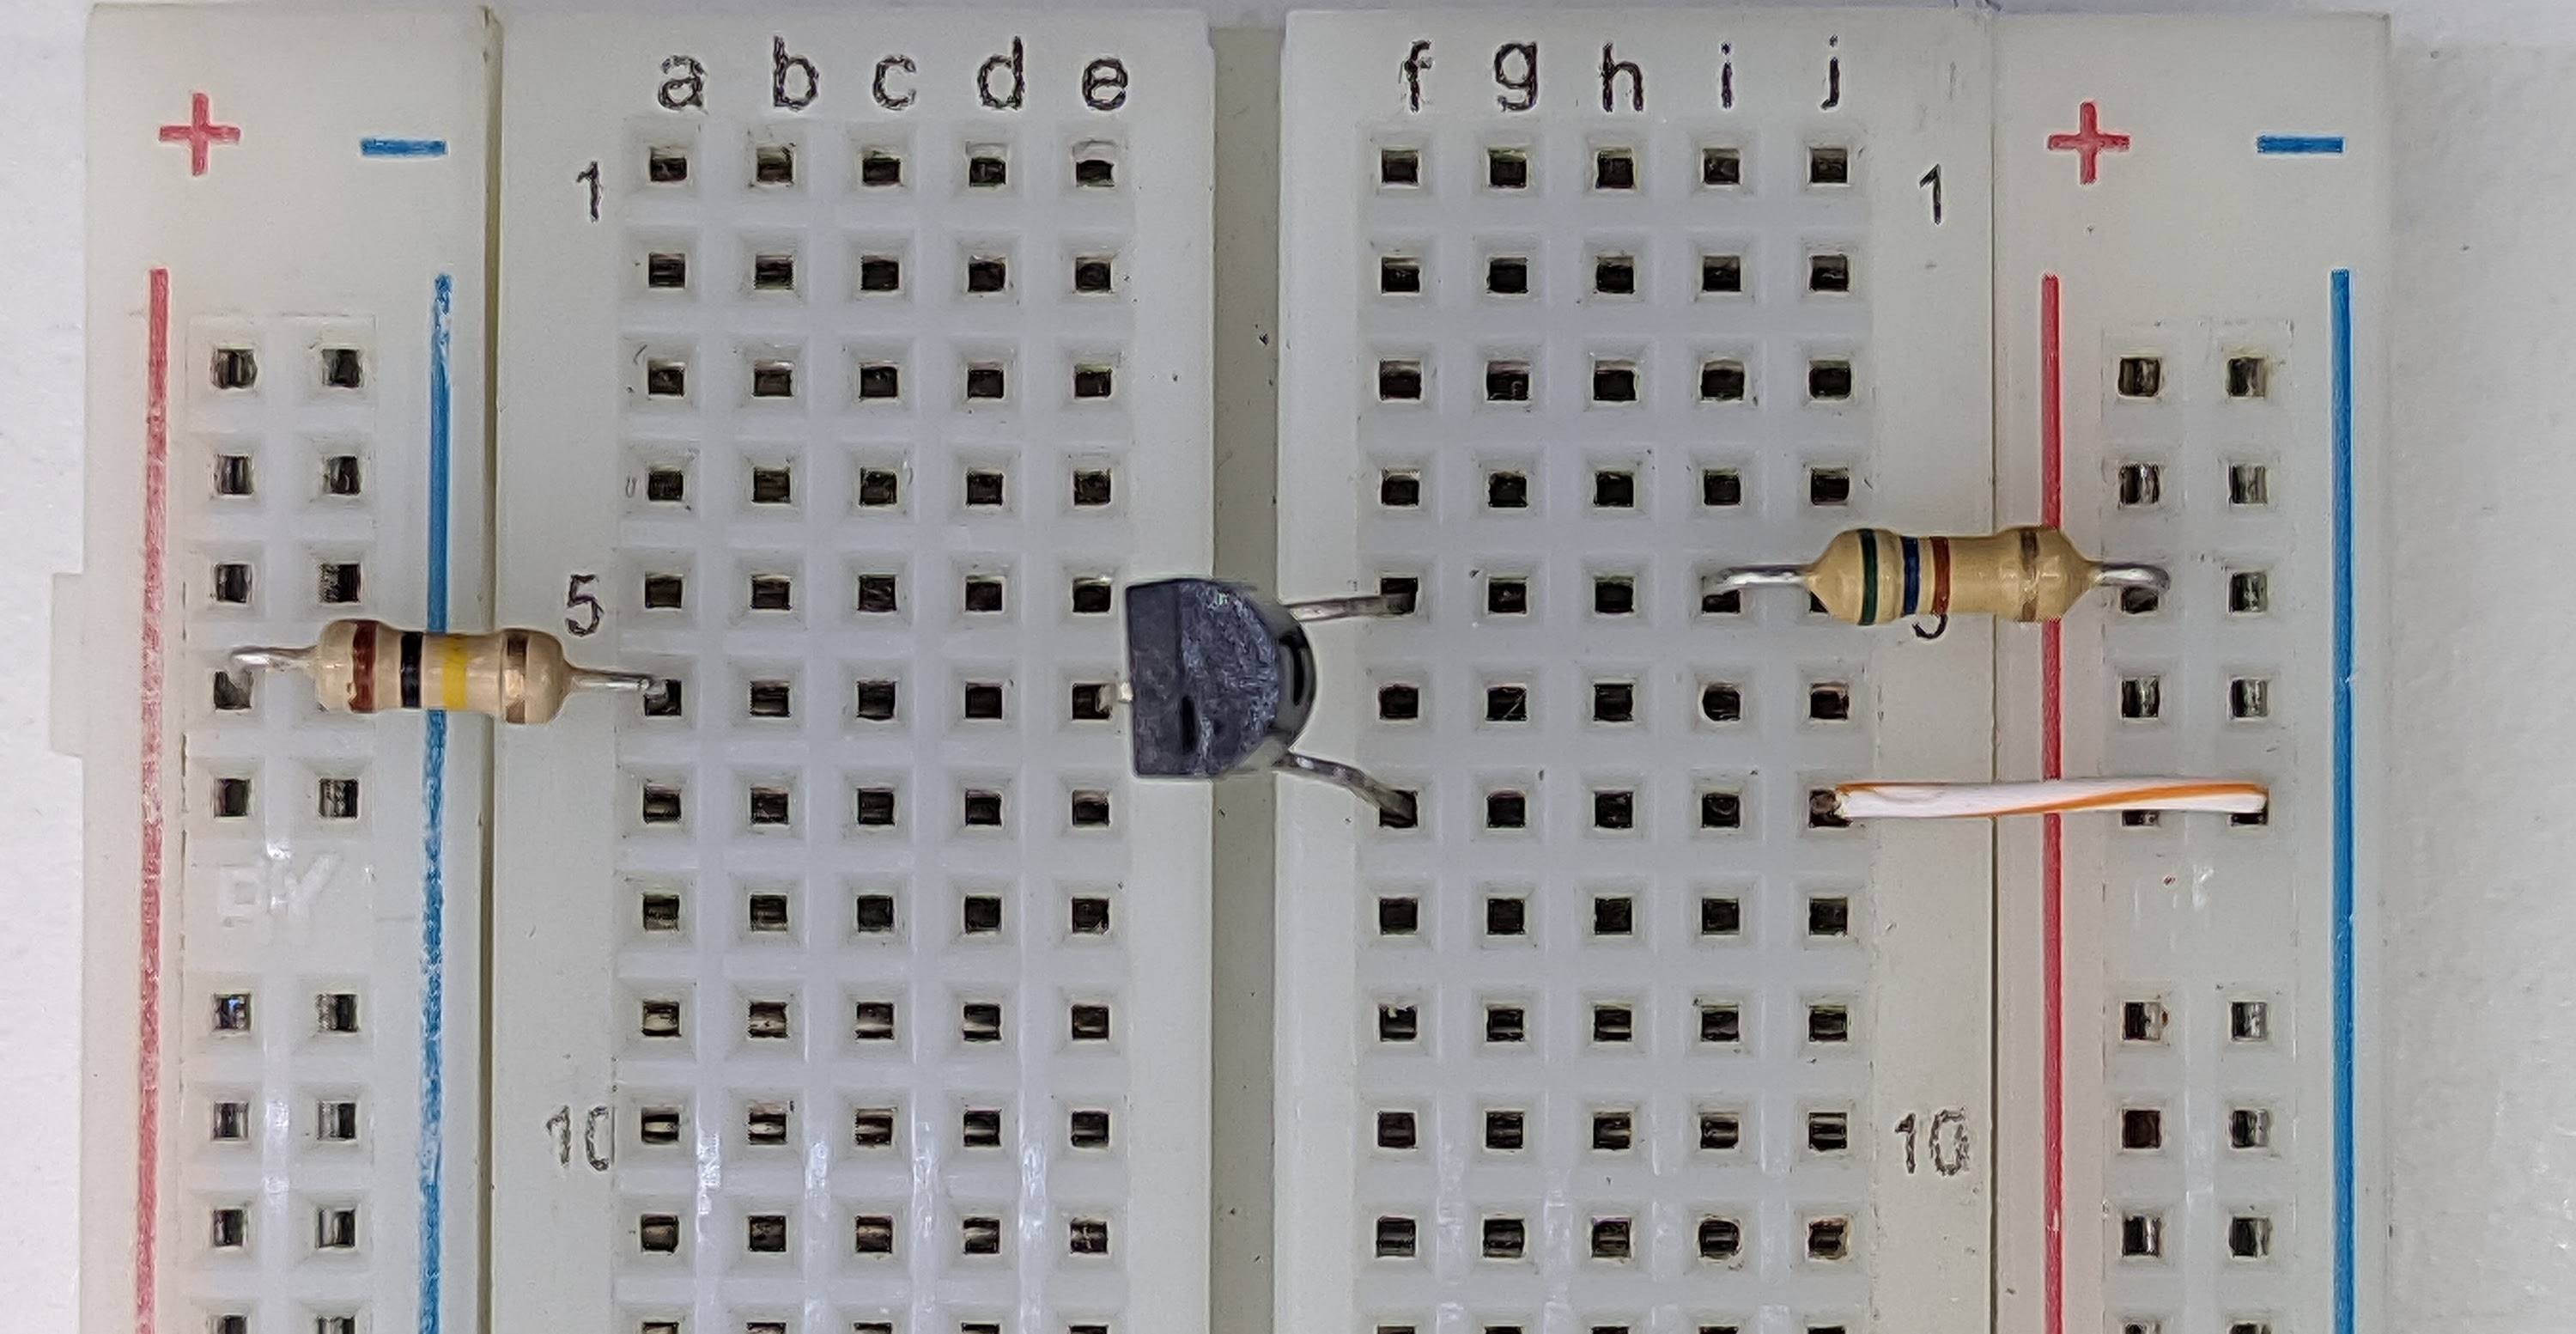
\includegraphics[width=1\textwidth]{tp3/pictures/prot_crkt-2_3.jpg}
            \caption{Circuito implementado.}
 
        \end{minipage}
                    \begin{minipage}{0.5\textwidth}
            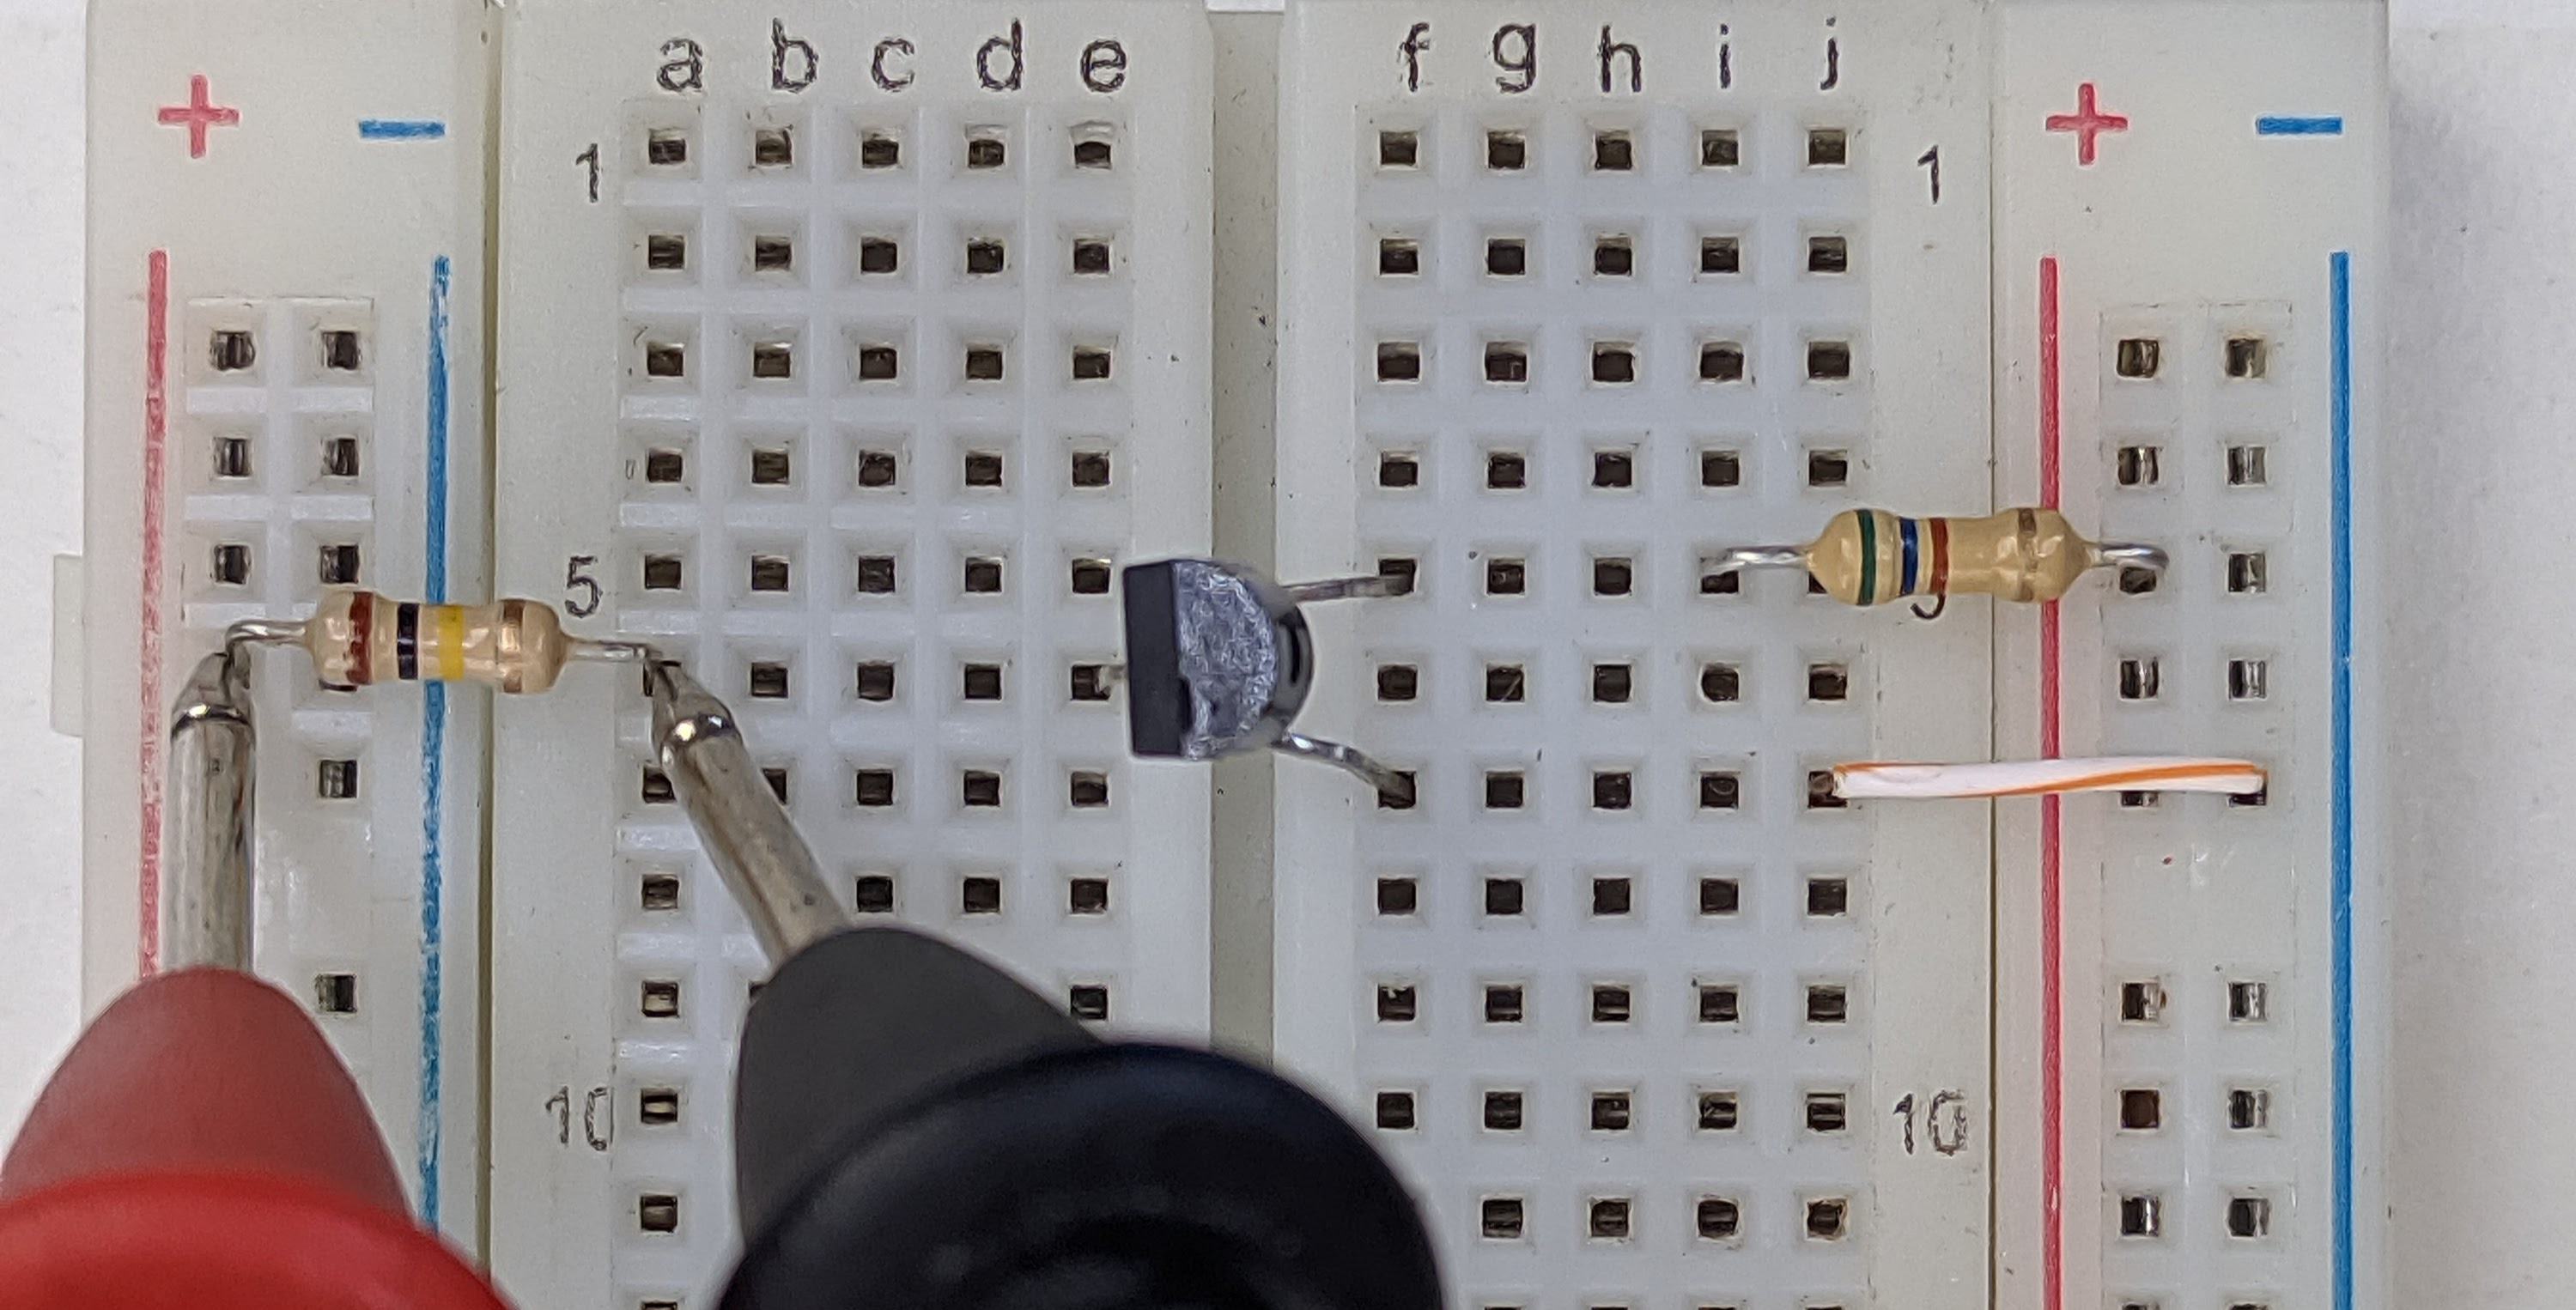
\includegraphics[width=1\textwidth]{tp3/pictures/prot_crkt-2_3_Vrb.jpg}
            \caption{Mediciones de $V_{RB}$.}

        \end{minipage}
        
 
    \end{figure}

  A continuacion se muestran imagenes que se tomaron durante la medicion:


   \begin{figure}[!ht]

        \begin{minipage}{0.5\textwidth}
            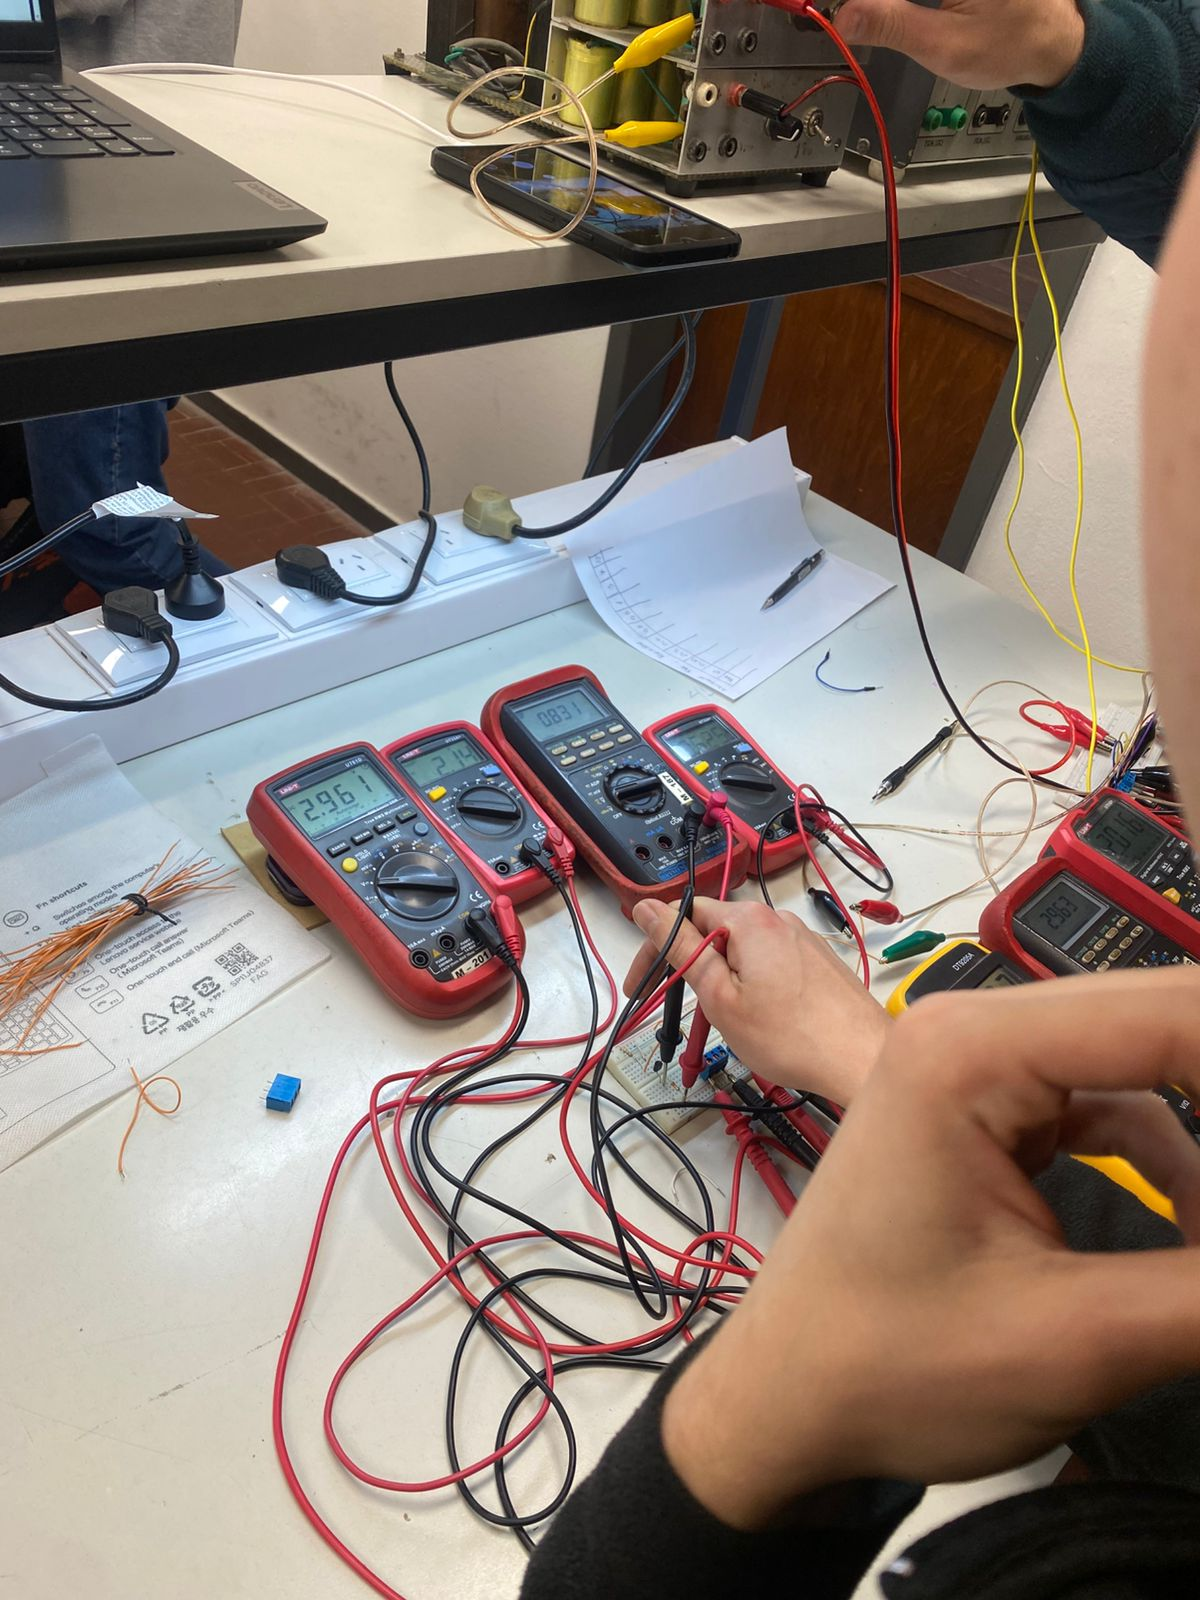
\includegraphics[width=1\textwidth]{tp3/pictures/setup_crkt-3_1.jpeg}
            \caption{Mediciones del circuito.}
 
        \end{minipage}
                    \begin{minipage}{0.5\textwidth}
            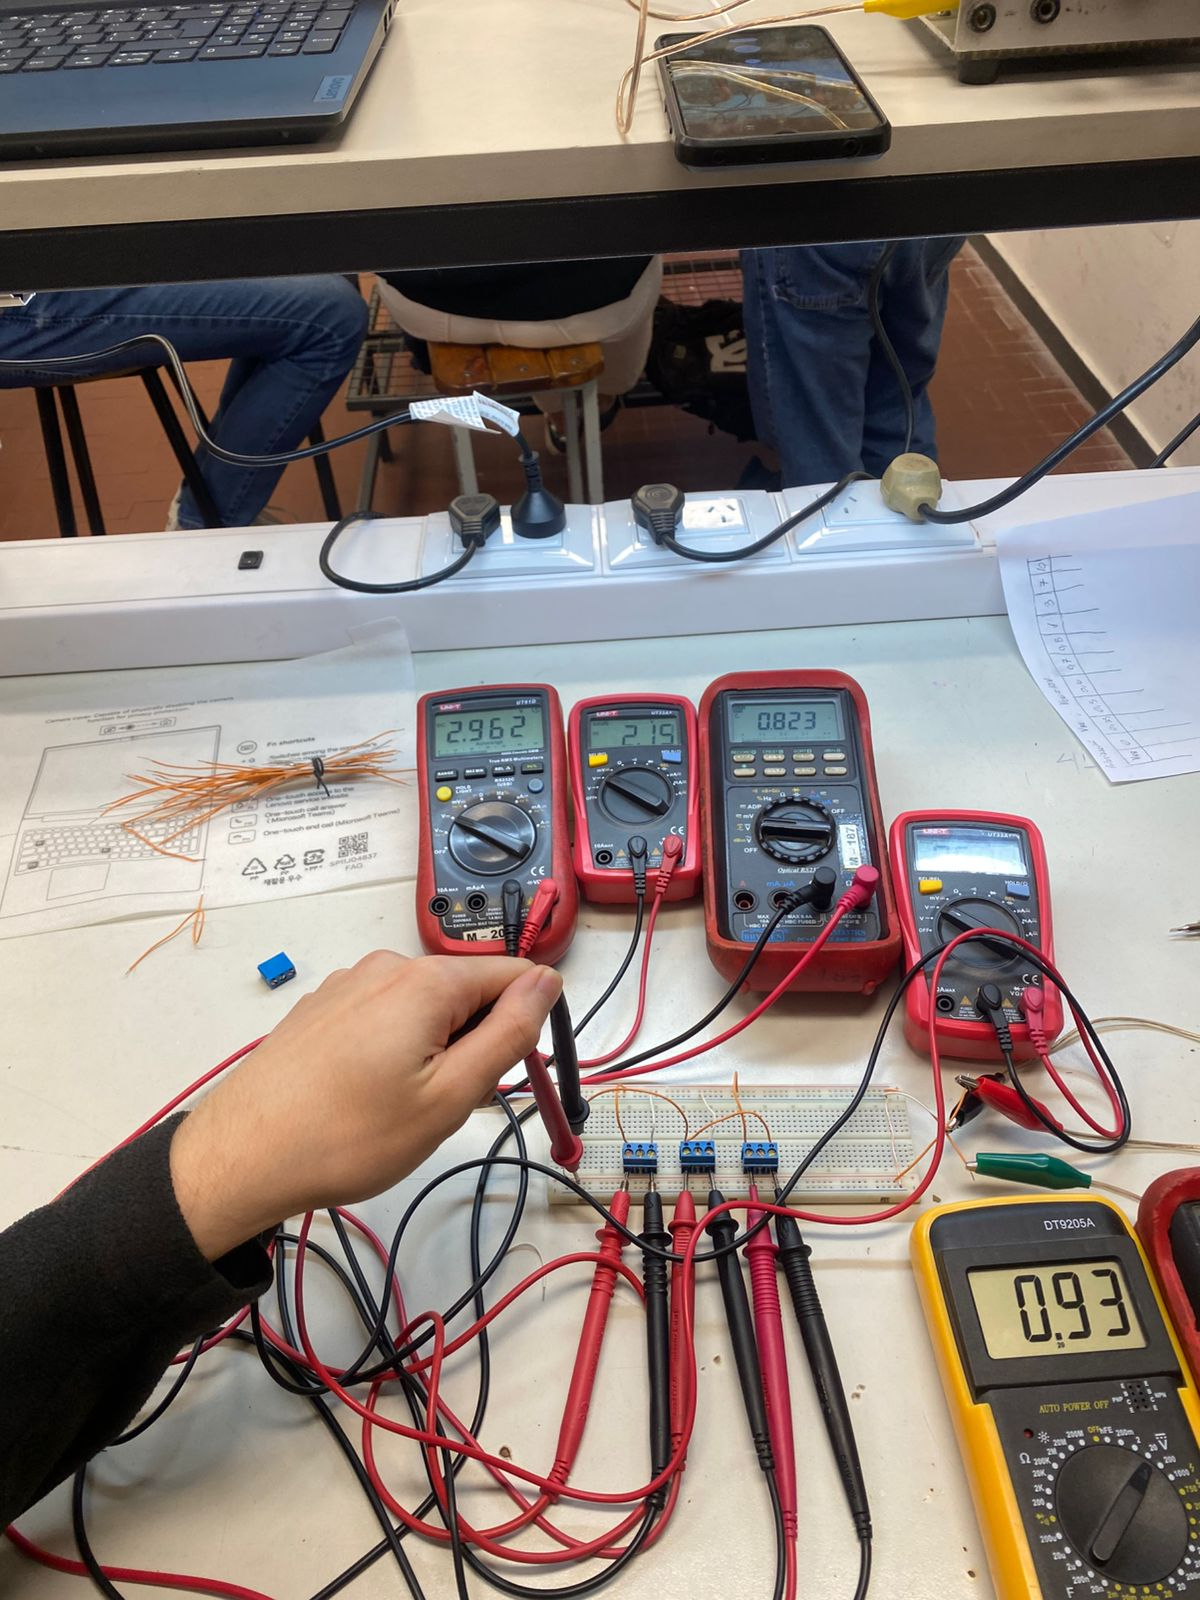
\includegraphics[width=1\textwidth]{tp3/pictures/setup_crkt-3_2.jpeg}
            \caption{Mediciones del circuito $V_{be}$.}

        \end{minipage}
        
 
    \end{figure}

\newpage
    \begin{table}
    \centering
    \resizebox{\textwidth}{!}{
    \begin{tabular}{*{11}{|c}|}
      \hline
      \multirow{2}{4em}{\centering $V_{CC}$} & \multicolumn{2}{c|}{$I_B = 0 \, A$} & \multicolumn{2}{c|}{$I_B = 10 \, \mu A$} & \multicolumn{2}{c|}{$I_B = 15 \, \mu A$} & \multicolumn{2}{c|}{$I_B = 20 \, \mu A$} & \multicolumn{2}{c|}{$I_B = 25 \, \mu A$}\\ \cline{2-11}
                  & $I_C$         & $V_{CE}$      & $I_C$           & $V_{CE}$      & $I_C$           & $V_{CE}$      & $I_C$           & $V_{CE}$      & $I_C$           & $V_{CE}$\\ \hline
      $0 \, V$    & $71 \, nA$    & $0 \, V$      & $12 \, \mu A$   & $0 \, V$      & $3 \, \mu A$    & $0 \, V$      & $8 \, \mu A$    & $0 \, V$      & $16 \, \mu A$   & $0 \, V$     \\ \hline
      $0.25 \, V$ & $160 \, nA$   & $0.257 \, V$  & $308 \, \mu A$  & $0.08 \, V$   & $335 \, \mu A$  & $0.069 \, V$  & $337 \, \mu A$  & $0.059 \, V$  & $337 \, \mu A$  & $0.054 \, V$ \\ \hline
      $0.5 \, V$  & $267 \, nA$   & $0.493 \, V$  & $698 \, \mu A$  & $0.108 \, V$  & $735 \, \mu A$  & $0.094 \, V$  & $723 \, \mu A$  & $0.083 \, V$  & $760 \, \mu A$  & $0.075 \, V$ \\ \hline
      $1 \, V$    & $267 \, nA$   & $1 \, V$      & $1.54 \, mA$    & $0.151 \, V$  & $1.5 \, mA$     & $0.122 \, V$  & $1.63 \, mA$    & $0.112 \, V$  & $1.68 \, mA$    & $0.150 \, V$ \\ \hline
      $2 \, V$    & $232 \, nA$   & $2 \, V$      & $3 \, mA$       & $0.273 \, V$  & $3.31 \, mA$    & $0.173 \, V$  & $3.4 \, mA$     & $0.151 \, V$  & $3.36 \, mA$    & $0.138 \, V$ \\ \hline
      $5 \, V$    & $517 \, nA$   & $5 \, V$      & $1.95 \, mA$    & $3.96 \, V$   & $2.56 \, mA$    & $3.56 \, V$   & $3.1 \, mA$     & $3.26 \, V$   & $7.85 \, mA$    & $0.553 \, V$ \\ \hline
      $10 \, V$   & $1 \, \mu A$  & $10 \, V$     & $1.69 \, mA$    & $9.14 \, V$   & $2.39 \, mA$    & $8.75 \, V$   & $3.3 \, mA$     & $8.19 \, V$   & $5.34 \, mA$    & $7.19 \, V$  \\ \hline
    \end{tabular}
    }
  \end{table}

\newpage

  \section{Conclusion}

    A partir del análisis experimental y simulado de las curvas características del transistor BJT, se identificaron claramente sus tres regiones de operación: corte, activa y saturación. Al mantener fija la corriente de base $I_B$ y barrer la tensión colector-emisor $V_{CE}$, se obtuvieron curvas $I_C$ vs.\ $V_{CE}$ que reflejan el comportamiento esperado del dispositivo.
    
    En la región activa se verificó una relación aproximadamente lineal entre $I_C$ e $I_B$, confirmando el modelo de amplificación controlada por corriente. En saturación, se observó que el transistor limita su capacidad de amplificación, mientras que en corte la corriente de colector fue prácticamente nula. La comparación entre los resultados de simulación y laboratorio mostró buena concordancia con la teoría, permitiendo validar el modelo del BJT como amplificador de señal o como conmutador, según el punto de operación elegido.
